\documentclass[11pt,a4paper]{article}
\usepackage{geometry}
\usepackage{graphicx}
\usepackage{amsmath}
\usepackage{listings}
\usepackage{xcolor}
\usepackage{float}
\usepackage{caption}
\usepackage{subcaption}
\usepackage{textcomp}
\usepackage[utf8]{inputenc}
\usepackage{array}

\geometry{margin=2.5cm}

% MATLAB code style
\lstdefinestyle{matlab}{
    language=Matlab,
    basicstyle=\small\ttfamily,
    keywordstyle=\color{blue},
    commentstyle=\color{green!60!black},
    stringstyle=\color{red},
    numberstyle=\tiny\color{gray},
    breaklines=true,
    frame=single,
    backgroundcolor=\color{gray!10},
    numbers=left,
    numbersep=5pt,
    showstringspaces=false,
    tabsize=2
}

\title{EN3563 Robotics Laboratory Experiment 02\\
Answer Sheet}
\author{Index No: 220148G \hspace{3cm}}
\date{}

\begin{document}

\maketitle

\section{Homogeneous Transformation Matrix $H_1^0$ for Task 3.4}

The homogeneous transformation matrix $H_1^0$ represents the transformation from frame $\{0\}$ to frame $\{1\}$, where frame $\{1\}$ is rotated 90\textdegree{} about the z-axis and translated by vector $q^0 = [2, 1, 1]^T$.

$$H_1^0 = \begin{bmatrix}
0 & -1 & 0 & 2 \\
1 & 0 & 0 & 1 \\
0 & 0 & 1 & 1 \\
0 & 0 & 0 & 1
\end{bmatrix}$$

\section{MATLAB Code for Tasks 3.1 to 3.6}

\begin{lstlisting}[style=matlab, caption={MATLAB Code for Tasks 3.1-3.6}]
clear; close all; clc;

% 3.1 - Visualize coordinate system {0}
figure; hold on; grid on; axis([0 4 0 4 0 3]); view(35,25);
trplot(eye(4),'frame','0','color','b');

% 3.2 - Obtain rotation matrix and translation vector
q0  = [2; 1; 1];           % translation vector t1_0
R1_0 = rotz(pi/2);         % 90 degrees about z-axis
t1_0 = q0;

% 3.3 - Visualize q0 using blue color
quiver3(0,0,0, q0(1),q0(2),q0(3), 0, 'Color','b');

% Create cube wireframe to show q0 vector endpoint
qx = q0(1); qy = q0(2); qz = q0(3);
C = [ 0  0  0;   qx 0  0;   qx qy 0;   0  qy 0;   
      0  0  qz;   qx 0  qz;   qx qy qz;   0  qy qz ];
E = [1 2; 2 3; 3 4; 4 1;   5 6; 6 7; 7 8; 8 5;   1 5; 2 6; 3 7; 4 8];
for k = 1:size(E,1)
    i = E(k,1); j = E(k,2);
    plot3([C(i,1) C(j,1)], [C(i,2) C(j,2)], [C(i,3) C(j,3)], 'b--');
end

% 3.4 - Obtain homogeneous transformation matrix H1_0
H1_0 = rt2tr(R1_0, t1_0);          % homogeneous transform
trplot(H1_0,'frame','1','color','r');
disp('H1_0 ='); disp(H1_0);

% 3.5 - Find p0 and visualize using green color
p1 = [0.5; 0.8; 0.6];             % define p1 in frame {1}
p0 = h2e(H1_0 * e2h(p1));          % p0 = H1_0 * p1 (homogeneous)
quiver3(0,0,0, p0(1), p0(2), p0(3), 0, 'Color','g');

% 3.6 - Visualize p1 using red color
u = R1_0 * p1;                    % p1 expressed in {0}
quiver3(q0(1),q0(2),q0(3), u(1),u(2),u(3), 0, 'Color','r');
\end{lstlisting}

\section{Final Output MATLAB Figure for Operations 3.1 to 3.6}

\begin{figure}[H]
    \centering
    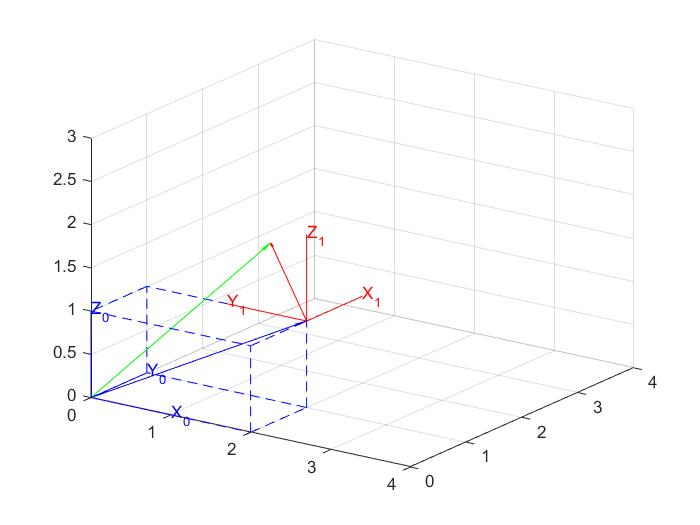
\includegraphics[width=0.8\textwidth]{figure_1.jpg}
    \caption{3D visualization showing coordinate frames \{0\} (blue) and \{1\} (red), position vector $q^0$ (blue arrow), transformed point $p^0$ (green arrow), and point $p^1$ (red arrow) from frame \{1\}}
\end{figure}

\section{Homogeneous Transformation Matrix $H_0^1$ for Task 3.8}

The inverse homogeneous transformation matrix $H_0^1$ represents the transformation from frame $\{1\}$ to frame $\{0\}$:

$$H_0^1 = (H_1^0)^{-1} = \begin{bmatrix}
0 & 1 & 0 & -1 \\
-1 & 0 & 0 & 2 \\
0 & 0 & 1 & -1 \\
0 & 0 & 0 & 1
\end{bmatrix}$$

\section{$t_0^1$ for Task 3.10}

The translation vector $t_0^1$ extracted from the homogeneous transformation matrix $H_0^1$:

$$t_0^1 = \begin{bmatrix} -1.0000 \\ 2.0000 \\ -1.0000 \end{bmatrix}$$

\section{MATLAB Code for Tasks 3.7 to 3.11}

\begin{lstlisting}[style=matlab, caption={MATLAB Code for Tasks 3.7-3.11}]
% 3.7 - New figure to visualize coordinate system {1} and p1
figure; hold on; grid on; axis([-4 2 -1 3 -2 2]); view(35,25);
trplot(eye(4),'frame','1','color','r');
quiver3(0,0,0, p1(1),p1(2),p1(3), 0, 'Color','r');

% 3.8 - Obtain homogeneous transformation matrix H0_1
H0_1 = inv(H1_0); 
disp('H0_1 ='); disp(H0_1);

% 3.9 - Visualize frame {0} with blue color
trplot(H0_1,'frame','0','color','b');

% 3.10 - Find t0_1 and visualize with blue color
[~, t0_1] = tr2rt(H0_1);
quiver3(0,0,0, t0_1(1), t0_1(2), t0_1(3), 0, 'Color','b'); 
fprintf('t0_1 = [%.4f %.4f %.4f]^T\n', t0_1);

% 3.11 - Visualize green arrow from tip of p1 to origin of frame {0}
d = t0_1 - p1;  % vector from p1 to origin of {0}
quiver3(p1(1), p1(2), p1(3), d(1), d(2), d(3), 0, 'Color','g');
\end{lstlisting}

\section{Final Output MATLAB Figure for Operations 3.7 to 3.11}

\begin{figure}[H]
    \centering
    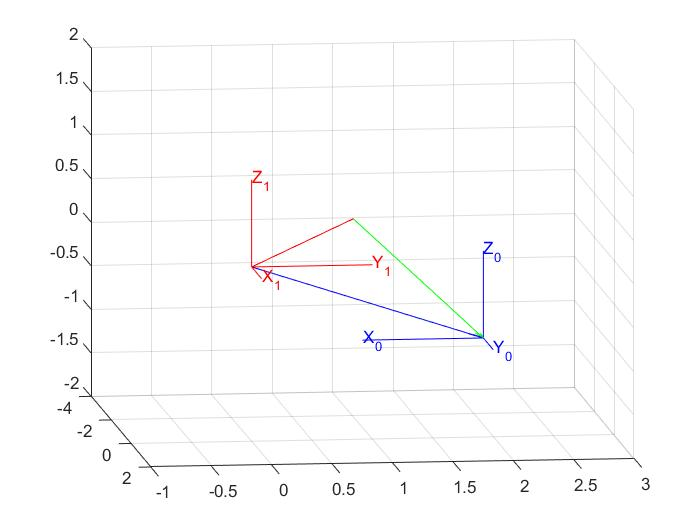
\includegraphics[width=0.8\textwidth]{figure 2.jpg}
    \caption{3D visualization from frame \{1\} perspective showing coordinate frame \{1\} (red), point $p^1$ (red arrow), coordinate frame \{0\} (blue), translation vector $t_0^1$ (blue arrow), and green arrow from tip of $p^1$ to origin of frame \{0\}}
\end{figure}

\section{Homogeneous Transformation Table}

\begin{table}[H]
\centering
\begin{tabular}{|p{3cm}|p{6cm}|p{4cm}|}
\hline
\textbf{Requirement} & \textbf{MATLAB Script to Satisfy Requirement} & \textbf{Homogeneous Transformation Matrix Result} \\
\hline
$o_0x_0y_0z_0$ to $o_1x_1y_1z_1$ & 
\begin{lstlisting}[style=matlab, basicstyle=\tiny\ttfamily, frame=none, numbers=none]
H1_0 = rt2tr(eye(3), 
   [-0.5; 1.5; 1.0]);
\end{lstlisting} & 
$\begin{bmatrix}
1 & 0 & 0 & -0.5 \\
0 & 1 & 0 & 1.5 \\
0 & 0 & 1 & 1.0 \\
0 & 0 & 0 & 1
\end{bmatrix}$ \\
\hline
$o_0x_0y_0z_0$ to $o_2x_2y_2z_2$ & 
\begin{lstlisting}[style=matlab, basicstyle=\tiny\ttfamily, frame=none, numbers=none]
H2_0 = rt2tr(eye(3), 
   [-0.5; 1.5; 1.1]);
\end{lstlisting} & 
$\begin{bmatrix}
1 & 0 & 0 & -0.5 \\
0 & 1 & 0 & 1.5 \\
0 & 0 & 1 & 1.1 \\
0 & 0 & 0 & 1
\end{bmatrix}$ \\
\hline
$o_0x_0y_0z_0$ to $o_3x_3y_3z_3$ & 
\begin{lstlisting}[style=matlab, basicstyle=\tiny\ttfamily, frame=none, numbers=none]
H3_0 = rt2tr(rotx(pi), 
   [-0.5; 1.5; 3.0]);
\end{lstlisting} & 
$\begin{bmatrix}
1 & 0 & 0 & -0.5 \\
0 & -1 & 0 & 1.5 \\
0 & 0 & -1 & 3.0 \\
0 & 0 & 0 & 1
\end{bmatrix}$ \\
\hline
\end{tabular}
\caption{Homogeneous transformation matrices for the 3D environment (Task 3.12)}
\end{table}

\begin{figure}[H]
    \centering
    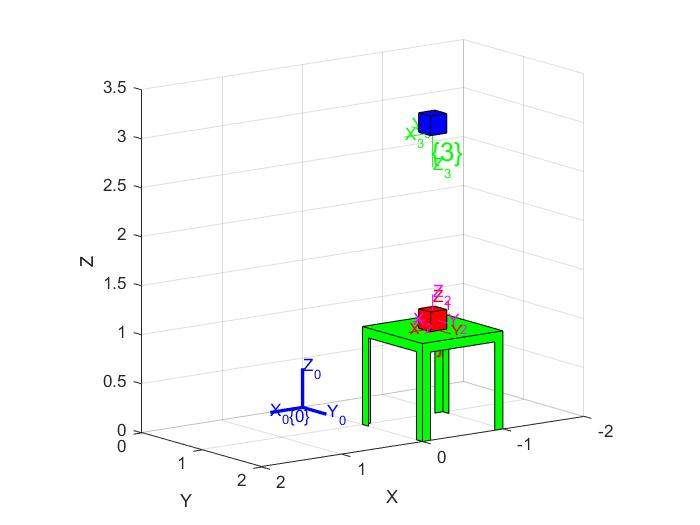
\includegraphics[width=0.8\textwidth]{figure_3.jpg}
    \caption{3D environment for visual servoing showing table (green), box (red), camera (blue), and coordinate frames \{0\}, \{1\}, \{2\}, \{3\}}
\end{figure}

\end{document}